\section{Dynamic White Box Testing}
\label{sec:DynamicWhiteBoxTesting}
To ensure the correctness of the Oasis Library we enforce dynamic white box testing (side 106 - 107, Software Testing - af Ron Patton) through unit tests. 
kilde: %http://aulas.carlosserrao.net/lib/exe/fetch.php?media=0910:1008-1987_ieee_standard_for_software_unit_testing.pdf
The library is used by all GIRAF applications this means that if a bug exists in the library there is a potential bug in all GIRAF application.
Therefore the library must be thoroughly tested to make sure that few or no bugs exists.

As this project have been developed using the agile development methods Scrum we have not devised a full test plan (side 263 - 275, Software Testing - af Ron Patton) as this is not needed.
As a part of Scrum we have been testing the code snippets before they have been marked as completed.
A decision has been made \autoref{sec:somewhereInTheLibSection} to make a full functioning library for this semester.
This decision means that the development time has to be prioritized and therefore the focus will be on test-to-pass tests (side 66, Software Testing - af Ron Patton).
This ensures that the library will function as intended, though there is no guarantee that the library will work if bad parameters are used.

\subsection{Test Design}
A test design (side 281 - 282, Software testing - af Ron Patton) have been elaborated for each method in the helper classes of the Oasis Library.
This way the library methods will be tested along with the database thus saving some time.
This means that the tests will be more efficient as more code will be tested in every test, but it has the drawback that if a bug is found more code will have to be investigated in order to locate the bug.

The test design in \autoref{tab:TestDesign_AuthenticateProfile} is for the \texttt{authenticateProfile()} method.
This test design tests if a profile can be authenticated.
This is an essential method for the whole GIRAF platform, and therefore it is tested both using test-to-pass and test-to-fail tests to ensure that this method is particular robust.

\begin{table}[htbp]
	\centering
		\begin{tabular}{| p{4.5cm} | m{9cm} |}
			\hline
			Identifier: 				& TD00001 \\ \hline
			Feature to be tested:		& Authenticate profile. \\ \hline
			Approach:					& An automated test will be made to authenticate a profile by its certificate. \\
										&	\begin{enumerate}
												\item Enter a profile with a specific certificate in the database.
												\item Authenticate the profile by its certificate.
											\end{enumerate} \\ \hline
			Test case identification: 	& Check valid certificate Test Case ID\# 00001 \\
										& Check too long certificates Test Case ID\# 00002 \\
										& Check too short certificates Test Case ID\# 00003 \\
										& Check invalid certificates Test Case ID\# 00004 \\ \hline
			Pass/fail criteria:			& All valid profile certificates that matches the certificate in the database must be accepted as well as all invalid certificates must be rejected. \\ \hline
		\end{tabular}
	\caption{Test Design for \texttt{authenticatingProfile()}.}
	\label{tab:TestDesign_AuthenticateProfile}
\end{table}

The test design in \autoref{tab:TestDesign_GetProfileById} is for the \texttt{getProfileById} method.
This is also a very important method for the whole GIRAF platform therefore it is tested with the same mix of test-to-pass and test-to-fail tests.
The test make sure that a profile can be found by its id and that negative id's and id's not in the database will not make it crash.

\begin{table}[htbp]
	\centering
		\begin{tabular}{| p{4.5cm} | m{9cm} |}
			\hline
			Identifier: 				& TD00002 \\ \hline
			Feature to be tested:		& Get profile by id. \\ \hline
			Approach:					& An automated test will be made in order to ensure that the Oasis Library supports getting a profile by its id from the database. \\
										&	\begin{enumerate}
												\item Add Profiles to the database.
												\item Get profile by id and verify the output.
											\end{enumerate} \\ \hline
			Test case identification: 	& Check valid id present in the database Test Case ID\# 00005 \\
										& Check id not in the database Test Case ID\# 00006 \\
										& Check negative id Test Case ID\# 00007 \\ \hline
			Pass/fail criteria:			& The profile matching the id should be returned else null should be returned. \\ \hline
		\end{tabular}
	\caption{Test Design for \texttt{getProfileById()}.}
	\label{tab:TestDesign_GetProfileById}
\end{table}

The test design in \autoref{tab:TestDesign_GetChildrenByGuardian} is for the \texttt{getChildrenByGuardian} method.
This test ensures that the method performs as intended under normal operation.
This is done with a single test-to-pass test, which tests if children associated to a guardian can be retrieved from the database.

\begin{table}[htbp]
	\centering
		\begin{tabular}{| p{4.5cm} | m{9cm} |}
			\hline
			Identifier: 				& TD00003 \\ \hline
			Feature to be tested:		& Get children by guardian. \\ \hline
			Approach:					& An automated test will be made to ensure that the Oasis Library supports getting all children associated with one guardian. \\
										&	\begin{enumerate}
												\item Children and guardians should be added to the database.
												\item Associations between some children and guardians should be made.
												\item Get children by guardian should be called and the output verified.
											\end{enumerate} \\ \hline
			Test case identification: 	& Check valid guardian with children associated Test Case ID\# 00008 \\ \hline
			Pass/fail criteria:			& The list of children should match the children associated with the guardian. \\ \hline
		\end{tabular}
	\caption{Test Design for get children by guardian.}
	\label{tab:TestDesign_GetChildrenByGuardian}
\end{table}

More test designs have been elaborated but have not be entered in the report due to the similarities and the large amount.
Those test designs look similar to the test design for the \texttt{getChildrenByGuardian} method.

\subsection{Test Cases}
One or more test case are created for each test design (side 283 - 285, Software testing - af Ron Patton).
Every test case is created in order to test a part of a method to ensure that the method performs as intended in the tested situation.

The test cases for the test designs in the prior Section can be seen in 
\autoref{tab:TestCase_ValidCertificateHandling}, 
\autoref{tab:TestCase_CertificateToShortHandling},
\autoref{tab:TestCase_CertificateToLongHandling},
\autoref{tab:TestCase_InvalidCertificateHandling},
\autoref{tab:TestCase_ValidIdHandling},
\autoref{tab:TestCase_InvalidIdHandling},
\autoref{tab:TestCase_NegativeIdHandling}, 
and \autoref{tab:TestCase_ValidGuardianWithChildrenAssociatedHandling}.

\begin{table}[htbp]
	\centering
		\begin{tabular}{| p{4.5cm} | m{9cm} |}
			\hline
			Identifier: 					& TC00001 \\ \hline
			Test item:						& Valid Certificate handling of the \texttt{authenticateProfile()} method. \\ \hline
			Input specification:			& A valid certificate. \\ \hline
			Output specification: 			& The model of the authenticated profile. \\ \hline
			Environmental needs:			& A database is needed and the profile model. \\ \hline
			Special procedural requirements	& None. \\ \hline
			Intercase dependencies:			& None. \\ \hline
		\end{tabular}
	\caption{Test Case for valid certificate handling of the \texttt{authenticateProfile()} method.}
	\label{tab:TestCase_ValidCertificateHandling}
\end{table}

\begin{table}[htbp]
	\centering
		\begin{tabular}{| p{4.5cm} | m{9cm} |}
			\hline
			Identifier: 					& TC00002 \\ \hline
			Test item:						& Certificate lenght too short handling of the \texttt{authenticateProfile()} method. \\ \hline
			Input specification:			& A certificate shorther than 200 chars. \\ \hline
			Output specification: 			& Null. \\ \hline
			Environmental needs:			& A database is needed and the profile model. \\ \hline
			Special procedural requirements	& None. \\ \hline
			Intercase dependencies:			& None. \\ \hline
		\end{tabular}
	\caption{Test Case for certificate lenght too long handling of the \texttt{authenticateProfile()} method.}
	\label{tab:TestCase_CertificateToShortHandling}
\end{table}

\begin{table}[htbp]
	\centering
		\begin{tabular}{| p{4.5cm} | m{9cm} |}
			\hline
			Identifier: 					& TC00003 \\ \hline
			Test item:						& Certificate lenght too long handling of the \texttt{authenticateProfile()} method. \\ \hline
			Input specification:			& A certificate longer than 200 chars. \\ \hline
			Output specification: 			& Null. \\ \hline
			Environmental needs:			& A database is needed and the profile model. \\ \hline
			Special procedural requirements	& None. \\ \hline
			Intercase dependencies:			& None. \\ \hline
		\end{tabular}
	\caption{Test Case for certificate lenght too long handling of the \texttt{authenticateProfile()} method.}
	\label{tab:TestCase_CertificateToLongHandling}
\end{table}

\begin{table}[htbp]
	\centering
		\begin{tabular}{| p{4.5cm} | m{9cm} |}
			\hline
			Identifier: 					& TC00004 \\ \hline
			Test item:						& Invalid Certificate handling of the \texttt{authenticateProfile()} method. \\ \hline
			Input specification:			& An invalid certificate. \\ \hline
			Output specification: 			& Null. \\ \hline
			Environmental needs:			& A database is needed and the profile model. \\ \hline
			Special procedural requirements	& None. \\ \hline
			Intercase dependencies:			& None. \\ \hline
		\end{tabular}
	\caption{Test Case for invalid certificate handling of the \texttt{authenticateProfile()} method.}
	\label{tab:TestCase_InvalidCertificateHandling}
\end{table}

\begin{table}[htbp]
	\centering
		\begin{tabular}{| p{4.5cm} | m{9cm} |}
			\hline
			Identifier: 					& TC00005 \\ \hline
			Test item:						& Valid id present in the database handling of the \texttt{getProfileById()} method. \\ \hline
			Input specification:			& A valid id. \\ \hline
			Output specification: 			& The profile matching the id. \\ \hline
			Environmental needs:			& A database is needed and the profile model. \\ \hline
			Special procedural requirements	& None. \\ \hline
			Intercase dependencies:			& None. \\ \hline
		\end{tabular}
	\caption{Test Case for valid id handling of the \texttt{getProfileById()} method.}
	\label{tab:TestCase_ValidIdHandling}
\end{table}

\begin{table}[htbp]
	\centering
		\begin{tabular}{| p{4.5cm} | m{9cm} |}
			\hline
			Identifier: 					& TC00006 \\ \hline
			Test item:						& Invalid id present not present in the database handling of the \texttt{getProfileById()} method. \\ \hline
			Input specification:			& An invalid id. \\ \hline
			Output specification: 			& Null. \\ \hline
			Environmental needs:			& A database is needed and the profile model. \\ \hline
			Special procedural requirements	& None. \\ \hline
			Intercase dependencies:			& None. \\ \hline
		\end{tabular}
	\caption{Test Case for invalid id handling of the \texttt{getProfileById()} method.}
	\label{tab:TestCase_InvalidIdHandling}
\end{table}

\begin{table}[htbp]
	\centering
		\begin{tabular}{| p{4.5cm} | m{9cm} |}
			\hline
			Identifier: 					& TC00007 \\ \hline
			Test item:						& Negative id handling of the \texttt{getProfileById()} method. \\ \hline
			Input specification:			& A negative id. \\ \hline
			Output specification: 			& Null. \\ \hline
			Environmental needs:			& A database is needed and the profile model. \\ \hline
			Special procedural requirements	& None. \\ \hline
			Intercase dependencies:			& None. \\ \hline
		\end{tabular}
	\caption{Test Case for negative id handling of the \texttt{getProfileById()} method.}
	\label{tab:TestCase_NegativeIdHandling}
\end{table}

\begin{table}[htbp]
	\centering
		\begin{tabular}{| p{4.5cm} | m{9cm} |}
			\hline
			Identifier: 					& TC00008 \\ \hline
			Test item:						& Valid guardian with children associated handling of the \texttt{getChildrenByGuardian()} method. \\ \hline
			Input specification:			& A valid guardian. \\ \hline
			Output specification: 			& A list of associated children. \\ \hline
			Environmental needs:			& A database is needed and the profile model. \\ \hline
			Special procedural requirements	& None. \\ \hline
			Intercase dependencies:			& None. \\ \hline
		\end{tabular}
	\caption{Test Case for valid guardian with children associated handling of the \texttt{getChildrenByGuardian()} method.}
	\label{tab:TestCase_ValidGuardianWithChildrenAssociatedHandling}
\end{table}

\subsection{Test Results}
All the tests cases have led to the construction of 89 unit tests which have helped in the development of the library.
The tests have been split up into three parts: Initialization, execution, and assertion.

\begin{Java}{The \texttt{testAuthenticateProfileWithValidCertificate()} method.}{lst:testAuthenticateProfileWithValidCertificate}
public void testAuthenticateProfileWithValidCertificate() {
	Random rnd = new Random();
	StringBuilder cert = new StringBuilder();
	for (int i = 0; i < 200; i++)
	{
		cert.append((char)(rnd.nextInt(26) + 97));
	}
	String certificate = cert.toString();
	Profile expectedProfile = new Profile("Test", "Profile", null, Profile.pRoles.GUARDIAN.ordinal(), 12345678, null, null);

	long id = mActivity.helper.profilesHelper.insertProfile(expectedProfile);
	expectedProfile.setId(id);
	
	mActivity.helper.profilesHelper.setCertificate(certificate, expectedProfile);

	Profile actualProfile = mActivity.helper.profilesHelper.authenticateProfile(certificate);

	assertEquals("Should return profile; Test Profile", expectedProfile, actualProfile);
}
\end{Java}


\begin{figure}[htbp]
	\centering
		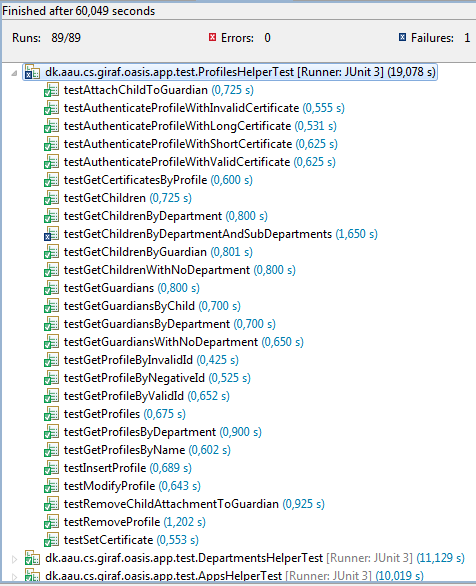
\includegraphics[width=\textwidth]{Images/unit_testing/profile_helper_tests.PNG}
	\caption{The result of the \texttt{profilesHelper} tests.}
	\label{fig:profile_helper_tests}
\end{figure}

\begin{figure}[htbp]
	\centering
		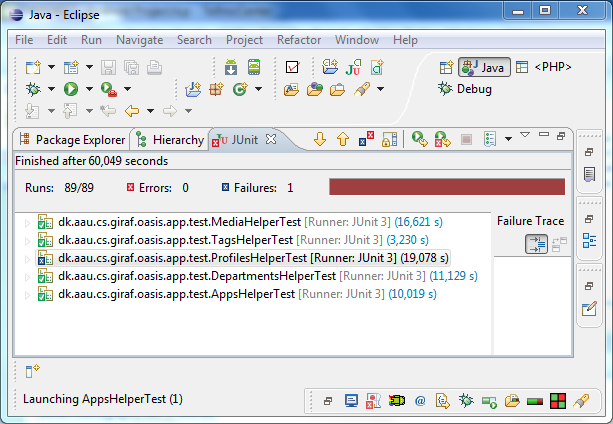
\includegraphics[width=\textwidth]{Images/unit_testing/all_tests.PNG}
	\caption{The result of all the performed unit tests.}
	\label{fig:all_tests}
\end{figure}

\begin{figure}[htbp]
	\centering
		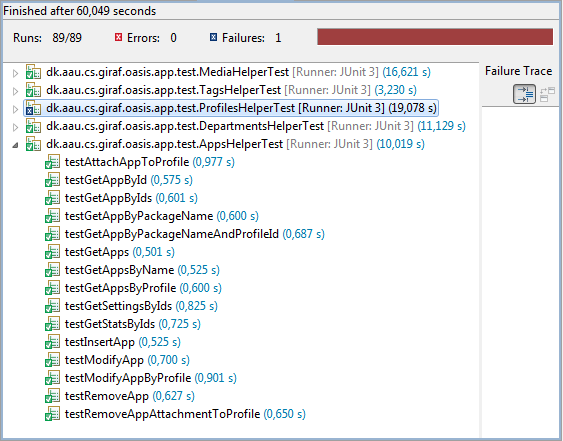
\includegraphics[width=\textwidth]{Images/unit_testing/app_helper_tests.PNG}
	\caption{The result of the \texttt{appsHelper} tests.}
	\label{fig:app_helper_tests}
\end{figure}

\begin{figure}[htbp]
	\centering
		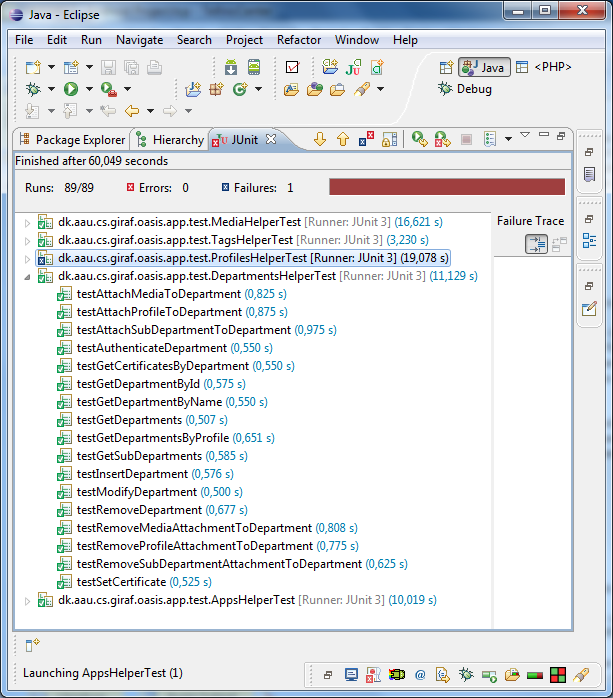
\includegraphics[width=\textwidth]{Images/unit_testing/department_helper_tests.PNG}
	\caption{The result of the \texttt{departmentHelper} tests.}
	\label{fig:department_helper_tests}
\end{figure}

\begin{figure}[htbp]
	\centering
		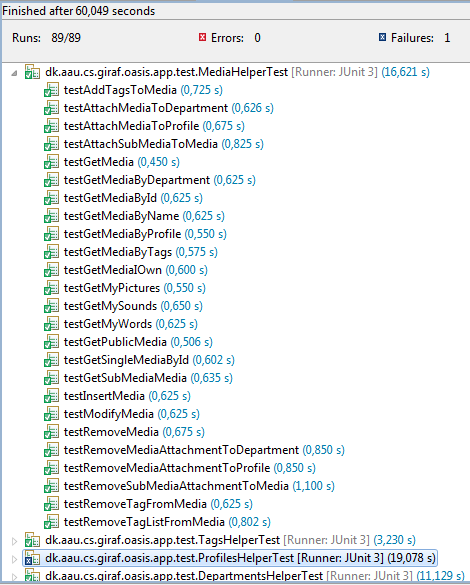
\includegraphics[width=\textwidth]{Images/unit_testing/media_helper_tests.PNG}
	\caption{The result of the \texttt{mediaHelper} tests.}
	\label{fig:media_helper_tests}
\end{figure}



\begin{figure}[htbp]
	\centering
		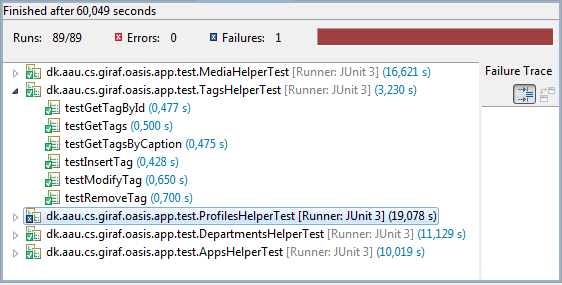
\includegraphics[width=\textwidth]{Images/unit_testing/tag_helper_tests.PNG}
	\caption{The result of the \texttt{tagsHelper} tests.}
	\label{fig:tag_helper_tests}
\end{figure}
